% XeLaTeX document
\documentclass[12pt,a4paper]{article}

% Редактируем: конфигурация, личные настройки: имя, название предмета и пр. для титульной страницы и метаданных документа здесь
\newcommand{\university}{Санкт-Петербургский политехнический университет Петра Великого}
\newcommand{\faculty}{Институт прикладной математики и механики}
\newcommand{\department}{Высшая школа прикладной математики и вычислительной физики}
\newcommand{\city}{Санкт-Петербург}
\newcommand{\num}{ №1}
\newcommand{\docname}{Отчёт по лабораторной работе}
\newcommand{\subject}{Название предмета}
\newcommand{\tutorname}{С. Г. Попов}
\newcommand{\studentname}{В. А. Тюльпин}
\newcommand{\group}{3630201/60101}

% Не редактируем: используемые пакеты
\usepackage{fontspec}
\setmainfont{FreeSerif}
\setsansfont{FreeSans}
\setmonofont{FreeMono}

\usepackage{polyglossia}
\usepackage{cite}
\usepackage[nottoc]{tocbibind}

% Не редактируем: параметры используемых пакетов и не только
% настройки polyglossia
\setdefaultlanguage{russian}
\setotherlanguages{english}

% % локализация
% \addto\captionsrussian{
% 	\renewcommand{\figurename}{Рисунок}%
% 	\renewcommand{\partname}{Глава}
% 	\renewcommand{\contentsname}{\centerline{Содержание}}
% 	\renewcommand{\listingscaption}{Листинг}
% }

% % основной шрифт документа
% \setmainfont{CMU Serif}
% \newfontfamily\cyrillicfont{CMU Serif}[Script=Cyrillic]

% водяной знак для обозначения статуса документа
% \newwatermark[allpages,color=red!5,angle=45,scale=3,xpos=0,ypos=0]{DRAFT}
\begin{document}
% Не редактируем: Титульная страница (формируется автоматически из заданной конфигурации)
\begin{titlepage}	% начало титульной страницы

	\begin{center}		% выравнивание по центру

		\large \university \\
		\large \faculty \\
		\large \department \\[6cm]
		% название института, затем отступ 6см

		\huge \subject \\[0.5cm] % название работы, затем отступ 0,5см
		\large \docname \num \\[5.1cm]
		% \large Тема работы\\[5cm]

	\end{center}


	\begin{flushright} % выравнивание по правому краю
		\begin{minipage}{0.25\textwidth} % врезка в половину ширины текста
			\begin{flushleft} % выровнять её содержимое по левому краю

				\large\textbf{Работу выполнил:}\\
				\large \studentname \\
				\large {Группа:} \group \\

				\large \textbf{Преподаватель:}\\
				\large \tutorname

			\end{flushleft}
		\end{minipage}
	\end{flushright}

	\vfill % заполнить всё доступное ниже пространство

	\begin{center}
		\large \city \\
		\large \the\year % вывести дату
	\end{center} % закончить выравнивание по центру

\end{titlepage} % конец титульной страницы

\vfill % заполнить всё доступное ниже пространство


% Не редактируем: Страница содержания (формируется автоматически из section, subsection и пр., указанных в content.tex)
% Содержание
\tableofcontents
\newpage



% Редактируем: всё остальное: вступление, др. этапы, заключение, приложение
\section*{Постановка задачи}
Необходимо сделать нормальный шаблон для отчётов в Политехе. Структура отчётов может быть разной, зависит от требования преподавателя, поэтому файл content.tex отдельно выделен от всех других в шаблоне и не делится на подчасти.
\addcontentsline{toc}{section}{Постановка задачи}

\newpage
\section{Заполнение шаблона}
\begin{itemize}
	\item Изменить \textbf{config.tex}: имя студента, название предмета и пр. параметры указаны именно там
	\item Заполнить \textbf{content.tex} - файл, который будет содержать весь текст отчёта, от вступления до заключения.
	\item Добавить используемую литературу (если есть) в \textbf{refs.bib}. Для удобного поиска источников можно воспользоваться Google Books. Использованные источники можно указывать с помощью команды \textbf{\\cite\{name\_of\_ref\}}
\end{itemize}
Далее представлены различные примеры.

\section{Теоретическая информация}
bash \cite{bash} \\

\section{Ход выполнения работы}

\subsection{Список}

\begin{itemize}
	\item первый элемент списка
	\item второй элемент списка
\end{itemize}


\subsection{Картинка}

\begin{figure}[H]
	\begin{center}
		
\includegraphics[scale=0.7]{sample}
		\caption{название картинки}
		\label{pic:pic_name} % название для ссылок внутри кода
	\end{center}
\end{figure}

Текст без отступа (следует за вставкой)

Новый параграф

\noindent Новый параграф с принудительно выключенным отступом


\subsection{Таблицы}

\begin{table}[H]
	\caption{Одна таблица}
	\begin{center}
		\begin{tabular*}{0.4\textwidth}{@{\extracolsep{\fill} } lcc}
			\toprule
			Element & First & Second \\
			\midrule
			One       & -    & -    \\
			Two       & -    & -    \\
			Three     & -    & -    \\
			Four      & -    & -    \\
			\bottomrule
		\end{tabular*}
		\label{tabular:tab_examp_1}
	\end{center}

	\caption{Другая таблица}
	\begin{center}
		\begin{tabular}{|l|c|r|}
			\hline
			top left & top center & top right \\ \hline
			bot left & bot center & bot right \\ \hline
		\end{tabular}
		\label{tabular:tab_examp_2}
	\end{center}
\end{table}

\begin{landscape}
	\subsection{Поворот страницы}
	Поворачиваем страницу, потому что можем.
	\begin{figure}[H]
		\centering
		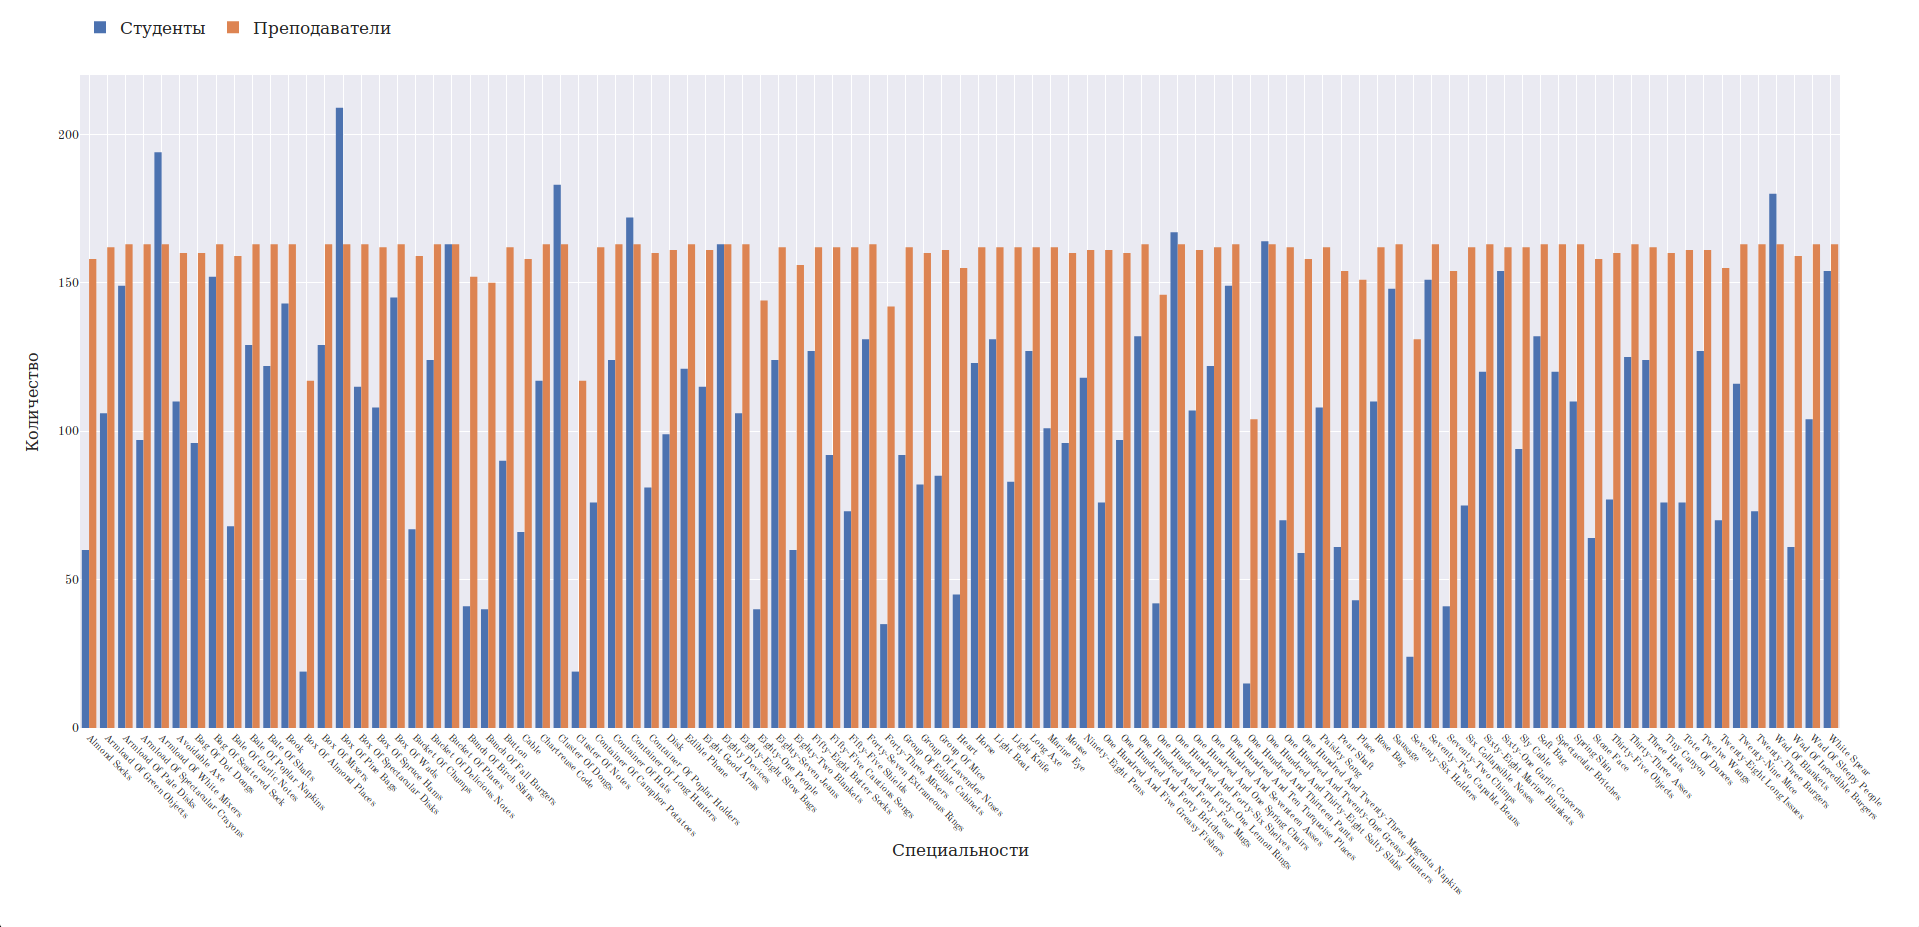
\includegraphics[width=25.5cm]{diagram}
		\caption{Да.}
	\end{figure}
\end{landscape}

\subsection{Листинг}
\begin{code}
	\inputminted[breaklines=true, xleftmargin=1em, linenos, frame=single, framesep=10pt, fontsize=\footnotesize, firstline=1, lastline=33]{haskell}{listings/Code.hs}
	\caption{Code.hs – функциональный код в массы!}
\end{code}

\newpage
\section*{Заключение}
\LaTeX\ удобен для создания отчётов, так как сам следит за нумерацией таблиц, рисунков, листингов и отсылок к ним (так, например, здесь всегда будет указан номер рисунка "sample" не зависимо от того, какой он (1,2 или другой) - это рисунок \ref{pic:pic_name}). Не менее важно что весь документ оформлен в едином стиле, а исходные материалы подключаются к отчёту, а не хранятся в нём. Всё это позволяет легко получить качественный отчёт без дополнительных трат на его офрмление.

Исключения, пожалуй, составляют таблицы, так как их значительно сложнее создавать кодом, нежели в графическом редакторе. Но здесь никто не запрещает использовать визуальные средства создания таблиц для \LaTeX\ .
\addcontentsline{toc}{section}{Заключение}

% Не редактируем: Страница библиографии (формируется автоматически из книжек, указанных в refs.bib и пометок \cite{имя_источника} в тексте)
\newpage
\printbibliography[title=Перечень использованных источников]
\addcontentsline{toc}{section}{Перечень использованных источников}
\end{document}
